\documentclass[11pt,a4paper]{article}
\usepackage[margin=1.9cm, top=2.1cm, bottom=2.0cm]{geometry}
\usepackage[T1]{fontenc}
\usepackage{lmodern}
\usepackage{amsmath,amssymb}
\usepackage{enumitem,booktabs,array,tabularx,multirow}
\usepackage[normalem]{ulem}
\usepackage{adjustbox}
\usepackage{xcolor}
\usepackage{fancyhdr,lastpage}
\usepackage[most]{tcolorbox}
\usepackage{tikz}
\usetikzlibrary{shapes.geometric,arrows.meta,positioning,calc}
\usepackage[hidelinks]{hyperref}
\setlength{\parindent}{0pt}
\setlength{\parskip}{4pt}
\renewcommand{\arraystretch}{1.25}
\emergencystretch=2em
\pagestyle{fancy}\fancyhf{}
\lhead{\small\textit{Course: CS420 -- Artificial Intelligence}}
\rhead{\small Practice Test 1}
\cfoot{\small Page \thepage\ of \pageref{LastPage}}
\renewcommand{\headrulewidth}{0.4pt}
% empty answer box (exam) / filled box (solution)
\newtcolorbox{ansbox}[1][]{enhanced, breakable, colback=white, colframe=black!55, boxrule=0.5pt, arc=0pt,
  left=5pt, right=5pt, top=3pt, bottom=3pt, before skip=3pt, after skip=6pt, #1}
\newtcolorbox{solbox}{enhanced, breakable, colback=blue!2!white, colframe=blue!50!black, boxrule=0.6pt, arc=0pt,
  left=6pt, right=6pt, top=4pt, bottom=4pt, before skip=3pt, after skip=8pt,
  fontupper=\color{black}}
\newcommand{\question}[1]{\par\medskip\noindent\textbf{Question #1.}\ }
\newcommand{\subq}[1]{\par\smallskip\noindent\textbf{#1}\ }
\newcommand{\T}{\textbf{\textcolor{green!45!black}{TRUE}}}
\newcommand{\F}{\textbf{\textcolor{red!70!black}{FALSE}}}

\tikzset{
  maxn/.style={draw, thick, regular polygon, regular polygon sides=3, minimum size=10.5mm, inner sep=0pt, font=\small},
  minn/.style={maxn, shape border rotate=180},
  chn/.style={draw, thick, circle, minimum size=9.5mm, inner sep=0pt, font=\small},
  leafn/.style={draw, rectangle, minimum width=5.5mm, minimum height=5.5mm, inner sep=1pt, font=\small},
  gone/.style={draw=black!25, text=black!35},
  cut/.style={red!80!black, very thick, dashed},
  sol/.style={text=blue!70!black, font=\small\bfseries},
}

\begin{document}


{\large\textbf{\textit{Course: CS420 -- Artificial Intelligence}}}\par
{\textbf{\textit{Midterm examination review -- Lectures 0 to 3}}}\par
\begin{center}{\Large\bfseries PRACTICE MIDTERM EXAMINATION -- TEST 1}\\[3pt]
{\small Duration: 120 minutes \quad$\cdot$\quad Closed book \quad$\cdot$\quad Calculator allowed}\end{center}
\noindent\rule{\linewidth}{0.6pt}

\noindent Full name: \rule{6.5cm}{0.3pt}\hfill Student ID: \rule{4cm}{0.3pt}\par\smallskip
{\small\textit{Unless a question says otherwise, ties are broken in alphabetical order (left-to-right in trees), and successors are generated in alphabetical order.}}\par
\question{1}\textit{The two-jug problem.} You have a 4-litre jug and a 3-litre jug, both initially empty, and a tap with unlimited water. You may fill a jug from the tap, empty a jug onto the ground, or pour one jug into the other until the source is empty or the destination is full. The goal is to have \emph{exactly 2 litres in the 4-litre jug}.
\subq{(a)}Consider a state as a tuple of values. Which values should be included in the tuple?
\begin{ansbox}[height=1.0cm]\end{ansbox}
\subq{(b)}Define the initial state and the goal state(s).
\begin{ansbox}[height=1.0cm]\end{ansbox}
\subq{(c)}Define the action function (preconditions and effects of every action).
\begin{ansbox}[height=2.0cm]\end{ansbox}
\subq{(d)}What is the action cost?
\begin{ansbox}[height=0.8cm]\end{ansbox}
\subq{(e)}What is the maximum number of states in the state space? How many are reachable from the initial state? Give a shortest solution.
\begin{ansbox}[height=2.0cm]\end{ansbox}
\question{2}Consider the undirected graph below; $S$ is the initial state and $G$ the goal state. Step costs are written on the edges and the heuristic $h$ next to the vertices. \begin{center}
\begin{adjustbox}{max width=\linewidth}
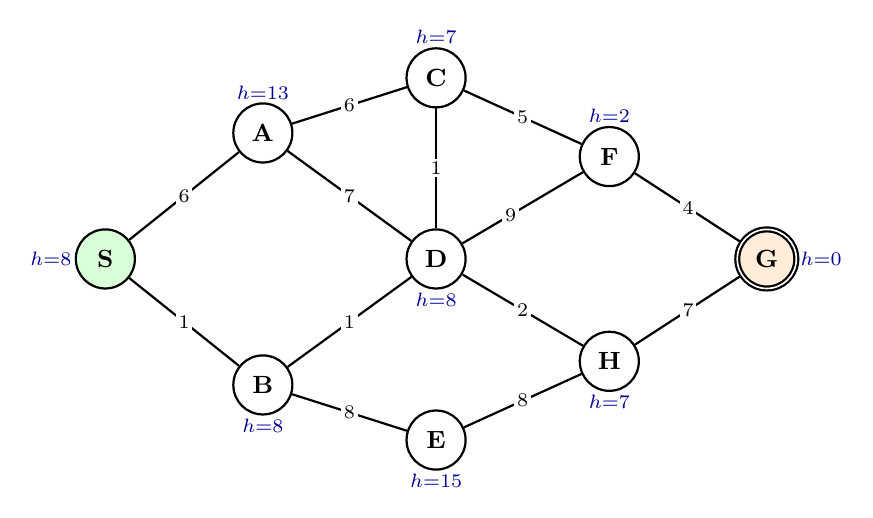
\begin{tikzpicture}[scale=1.0, every node/.style={transform shape}, gn/.style={draw, thick, circle, minimum size=7.5mm, inner sep=0pt, font=\small\bfseries}, ec/.style={font=\scriptsize, fill=white, inner sep=1pt}]
\node[gn, fill=green!15, label={[font=\scriptsize, text=blue!60!black, inner sep=1pt]left:$h{=}8$}] (S) at (0.00,0.00) {S};
\node[gn, label={[font=\scriptsize, text=blue!60!black, inner sep=1pt]above:$h{=}13$}] (A) at (2.00,1.60) {A};
\node[gn, label={[font=\scriptsize, text=blue!60!black, inner sep=1pt]below:$h{=}8$}] (B) at (2.00,-1.60) {B};
\node[gn, label={[font=\scriptsize, text=blue!60!black, inner sep=1pt]above:$h{=}7$}] (C) at (4.20,2.30) {C};
\node[gn, label={[font=\scriptsize, text=blue!60!black, inner sep=1pt]below:$h{=}8$}] (D) at (4.20,0.00) {D};
\node[gn, label={[font=\scriptsize, text=blue!60!black, inner sep=1pt]below:$h{=}15$}] (E) at (4.20,-2.30) {E};
\node[gn, label={[font=\scriptsize, text=blue!60!black, inner sep=1pt]above:$h{=}2$}] (F) at (6.40,1.30) {F};
\node[gn, label={[font=\scriptsize, text=blue!60!black, inner sep=1pt]below:$h{=}7$}] (H) at (6.40,-1.30) {H};
\node[gn, double, fill=orange!15, label={[font=\scriptsize, text=blue!60!black, inner sep=1pt]right:$h{=}0$}] (G) at (8.40,0.00) {G};
\draw[thick] (S) to[] node[ec, midway]{6} (A);
\draw[thick] (S) to[] node[ec, midway]{1} (B);
\draw[thick] (A) to[] node[ec, midway]{6} (C);
\draw[thick] (A) to[] node[ec, midway]{7} (D);
\draw[thick] (B) to[] node[ec, midway]{1} (D);
\draw[thick] (B) to[] node[ec, midway]{8} (E);
\draw[thick] (C) to[] node[ec, midway]{5} (F);
\draw[thick] (D) to[] node[ec, pos=0.4]{9} (F);
\draw[thick] (D) to[] node[ec, midway]{2} (H);
\draw[thick] (E) to[] node[ec, midway]{8} (H);
\draw[thick] (F) to[] node[ec, midway]{4} (G);
\draw[thick] (H) to[] node[ec, midway]{7} (G);
\draw[thick] (C) to[] node[ec, midway]{1} (D);
\end{tikzpicture}
\end{adjustbox}
\end{center}For each search strategy, (a) list, in order, the states \textbf{expanded}, (b) give the path found and (c) give the final content of the frontier (a state is expanded when it is removed from the frontier). Conventions: BFS, DFS and greedy best-first search test a state for the goal when it is \emph{generated} (so the goal is not expanded); UCS and A* test it when it is \emph{removed} from the frontier (graph search; a cheaper path to a frontier state replaces its entry). DFS avoids loops by remembering the states on the current path only. The path returned will not be accepted if the list of expanded states is wrong.

\begin{center}\small\begin{tabularx}{\linewidth}{|>{\raggedright}p{2.6cm}|>{\raggedright}X|>{\raggedright}p{3.6cm}|>{\raggedright\arraybackslash}p{2.6cm}|}\hline
\textbf{Algorithm} & \textbf{List of expanded states} & \textbf{Path returned} & \textbf{Final frontier}\\ \hline
Breadth-first search & & & \\[8mm] \hline
Uniform-cost search & & & \\[8mm] \hline
Depth-first search & & & \textit{(not asked)}\\[8mm] \hline
Greedy best-first search & & & \\[8mm] \hline
Graph-search A* & & & \\[8mm] \hline
\end{tabularx}\end{center}
\subq{(d)}Is $h$ admissible? Justify.
\begin{ansbox}[height=1.5cm]\end{ansbox}
\subq{(e)}Is $h$ consistent? Justify.
\begin{ansbox}[height=1.5cm]\end{ansbox}
\subq{(f)}Which of the five strategies returned an optimal path here, and which of them are guaranteed to do so?
\begin{ansbox}[height=1.5cm]\end{ansbox}
\clearpage
\question{3}Consider the 8-puzzle. Apply \emph{steepest-descent hill climbing} with the Manhattan-distance heuristic $h$ to the following pair of initial and goal states.\begin{center}Initial state\quad \begin{tabular}{|c|c|c|}\hline 1 & 2 & 3\\\hline 6 & -- & 4\\\hline 8 & 7 & 5\\\hline\end{tabular}\qquad\qquad Goal state\quad \begin{tabular}{|c|c|c|}\hline 1 & 2 & 3\\\hline 8 & -- & 4\\\hline 7 & 6 & 5\\\hline\end{tabular}\end{center}Your work should: draw the search tree including all successors of every expanded state (moves of the blank in the order Up, Down, Left, Right; do not regenerate the parent state), write the heuristic value of every node, and mark the path found.
\par\smallskip\noindent 
\begin{ansbox}[height=12.0cm]\end{ansbox}
\clearpage
\question{4}Consider the following game tree. The root is a MAX node and the search always visits children left to right (small grey numbers are leaf indices).\begin{center}
\begin{adjustbox}{max width=\linewidth}
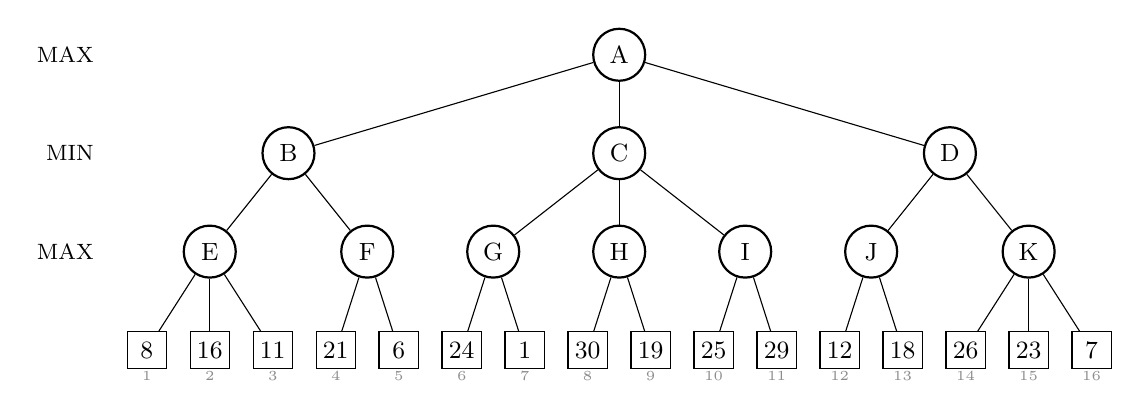
\begin{tikzpicture}[scale=1.0, every node/.style={transform shape}, gc/.style={draw, thick, circle, minimum size=6.6mm, inner sep=0pt, font=\small}, gl/.style={draw, rectangle, minimum width=5mm, minimum height=4.6mm, inner sep=1pt, font=\small}, gx/.style={draw=black!25, text=black!35}, val/.style={font=\footnotesize\bfseries, text=red!80!black, inner sep=1pt}]
\node[font=\footnotesize, anchor=east] at (-0.55,0.00) {MAX};
\node[font=\footnotesize, anchor=east] at (-0.55,-1.25) {MIN};
\node[font=\footnotesize, anchor=east] at (-0.55,-2.50) {MAX};
\node[gc] (n26) at (6.000,0.000) {A};
\node[gc] (n7) at (1.800,-1.250) {B};
\node[gc] (n3) at (0.800,-2.500) {E};
\node[gl, label={[font=\tiny, text=black!45, inner sep=1pt]below:1}] (n0) at (0.000,-3.750) {8};
\node[gl, label={[font=\tiny, text=black!45, inner sep=1pt]below:2}] (n1) at (0.800,-3.750) {16};
\node[gl, label={[font=\tiny, text=black!45, inner sep=1pt]below:3}] (n2) at (1.600,-3.750) {11};
\node[gc] (n6) at (2.800,-2.500) {F};
\node[gl, label={[font=\tiny, text=black!45, inner sep=1pt]below:4}] (n4) at (2.400,-3.750) {21};
\node[gl, label={[font=\tiny, text=black!45, inner sep=1pt]below:5}] (n5) at (3.200,-3.750) {6};
\node[gc] (n17) at (6.000,-1.250) {C};
\node[gc] (n10) at (4.400,-2.500) {G};
\node[gl, label={[font=\tiny, text=black!45, inner sep=1pt]below:6}] (n8) at (4.000,-3.750) {24};
\node[gl, label={[font=\tiny, text=black!45, inner sep=1pt]below:7}] (n9) at (4.800,-3.750) {1};
\node[gc] (n13) at (6.000,-2.500) {H};
\node[gl, label={[font=\tiny, text=black!45, inner sep=1pt]below:8}] (n11) at (5.600,-3.750) {30};
\node[gl, label={[font=\tiny, text=black!45, inner sep=1pt]below:9}] (n12) at (6.400,-3.750) {19};
\node[gc] (n16) at (7.600,-2.500) {I};
\node[gl, label={[font=\tiny, text=black!45, inner sep=1pt]below:10}] (n14) at (7.200,-3.750) {25};
\node[gl, label={[font=\tiny, text=black!45, inner sep=1pt]below:11}] (n15) at (8.000,-3.750) {29};
\node[gc] (n25) at (10.200,-1.250) {D};
\node[gc] (n20) at (9.200,-2.500) {J};
\node[gl, label={[font=\tiny, text=black!45, inner sep=1pt]below:12}] (n18) at (8.800,-3.750) {12};
\node[gl, label={[font=\tiny, text=black!45, inner sep=1pt]below:13}] (n19) at (9.600,-3.750) {18};
\node[gc] (n24) at (11.200,-2.500) {K};
\node[gl, label={[font=\tiny, text=black!45, inner sep=1pt]below:14}] (n21) at (10.400,-3.750) {26};
\node[gl, label={[font=\tiny, text=black!45, inner sep=1pt]below:15}] (n22) at (11.200,-3.750) {23};
\node[gl, label={[font=\tiny, text=black!45, inner sep=1pt]below:16}] (n23) at (12.000,-3.750) {7};
\draw (n26) -- (n7);
\draw (n26) -- (n17);
\draw (n26) -- (n25);
\draw (n7) -- (n3);
\draw (n7) -- (n6);
\draw (n3) -- (n0);
\draw (n3) -- (n1);
\draw (n3) -- (n2);
\draw (n6) -- (n4);
\draw (n6) -- (n5);
\draw (n17) -- (n10);
\draw (n17) -- (n13);
\draw (n17) -- (n16);
\draw (n10) -- (n8);
\draw (n10) -- (n9);
\draw (n13) -- (n11);
\draw (n13) -- (n12);
\draw (n16) -- (n14);
\draw (n16) -- (n15);
\draw (n25) -- (n20);
\draw (n25) -- (n24);
\draw (n20) -- (n18);
\draw (n20) -- (n19);
\draw (n24) -- (n21);
\draw (n24) -- (n22);
\draw (n24) -- (n23);
\end{tikzpicture}
\end{adjustbox}
\end{center}
\subq{(a)}Compute the final backed-up value of every node using the minimax algorithm (no alpha-beta pruning at this step). Which move should MAX make at the root?
\begin{center}\small \begin{tabular}{|l|c|c|c|c|c|c|c|c|c|c|c|}\hline
\textbf{Node} & \textbf{A} & \textbf{B} & \textbf{C} & \textbf{D} & \textbf{E} & \textbf{F} & \textbf{G} & \textbf{H} & \textbf{I} & \textbf{J} & \textbf{K}\\ \hline
Minimax & \phantom{00} & \phantom{00} & \phantom{00} & \phantom{00} & \phantom{00} & \phantom{00} & \phantom{00} & \phantom{00} & \phantom{00} & \phantom{00} & \phantom{00}\\[1.5mm] \hline
\end{tabular}\end{center}\begin{ansbox}[height=0.8cm]\end{ansbox}
\subq{(b)}Run alpha-beta pruning (children visited left to right). Give the value computed at every node (mark \textbf{X} if the node is never visited), cross out the pruned branches on the tree and briefly explain each case.
\begin{center}\small \begin{tabular}{|l|c|c|c|c|c|c|c|c|c|c|c|}\hline
\textbf{Node} & \textbf{A} & \textbf{B} & \textbf{C} & \textbf{D} & \textbf{E} & \textbf{F} & \textbf{G} & \textbf{H} & \textbf{I} & \textbf{J} & \textbf{K}\\ \hline
$\alpha$-$\beta$ & \phantom{00} & \phantom{00} & \phantom{00} & \phantom{00} & \phantom{00} & \phantom{00} & \phantom{00} & \phantom{00} & \phantom{00} & \phantom{00} & \phantom{00}\\[1.5mm] \hline
\end{tabular}\end{center}\begin{ansbox}[height=4.0cm]\end{ansbox}
\subq{(c)}Using the minimax values from (a), and without performing any alpha-beta calculation, rotate the children of each node at every level so that alpha-beta prunes as much as possible. Draw the new tree (keep the node letters).
\begin{ansbox}[height=5.5cm]\end{ansbox}
\clearpage
\question{5}Consider the following 4-ply game tree (MAX at the root).\begin{center}
\begin{adjustbox}{max width=\linewidth}
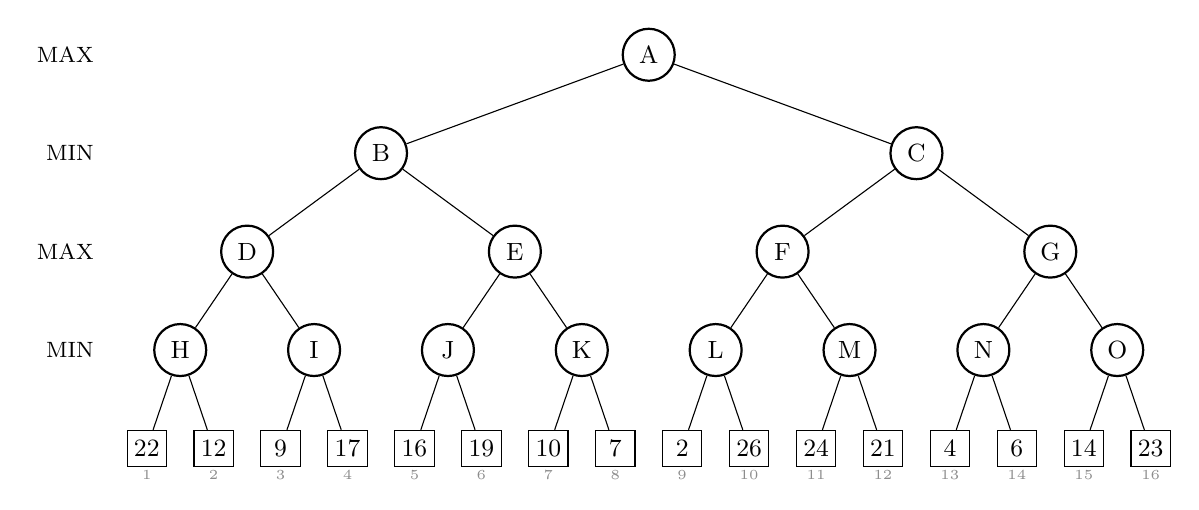
\begin{tikzpicture}[scale=1.0, every node/.style={transform shape}, gc/.style={draw, thick, circle, minimum size=6.6mm, inner sep=0pt, font=\small}, gl/.style={draw, rectangle, minimum width=5mm, minimum height=4.6mm, inner sep=1pt, font=\small}, gx/.style={draw=black!25, text=black!35}, val/.style={font=\footnotesize\bfseries, text=red!80!black, inner sep=1pt}]
\node[font=\footnotesize, anchor=east] at (-0.55,0.00) {MAX};
\node[font=\footnotesize, anchor=east] at (-0.55,-1.25) {MIN};
\node[font=\footnotesize, anchor=east] at (-0.55,-2.50) {MAX};
\node[font=\footnotesize, anchor=east] at (-0.55,-3.75) {MIN};
\node[gc] (n30) at (6.375,0.000) {A};
\node[gc] (n14) at (2.975,-1.250) {B};
\node[gc] (n6) at (1.275,-2.500) {D};
\node[gc] (n2) at (0.425,-3.750) {H};
\node[gl, label={[font=\tiny, text=black!45, inner sep=1pt]below:1}] (n0) at (0.000,-5.000) {22};
\node[gl, label={[font=\tiny, text=black!45, inner sep=1pt]below:2}] (n1) at (0.850,-5.000) {12};
\node[gc] (n5) at (2.125,-3.750) {I};
\node[gl, label={[font=\tiny, text=black!45, inner sep=1pt]below:3}] (n3) at (1.700,-5.000) {9};
\node[gl, label={[font=\tiny, text=black!45, inner sep=1pt]below:4}] (n4) at (2.550,-5.000) {17};
\node[gc] (n13) at (4.675,-2.500) {E};
\node[gc] (n9) at (3.825,-3.750) {J};
\node[gl, label={[font=\tiny, text=black!45, inner sep=1pt]below:5}] (n7) at (3.400,-5.000) {16};
\node[gl, label={[font=\tiny, text=black!45, inner sep=1pt]below:6}] (n8) at (4.250,-5.000) {19};
\node[gc] (n12) at (5.525,-3.750) {K};
\node[gl, label={[font=\tiny, text=black!45, inner sep=1pt]below:7}] (n10) at (5.100,-5.000) {10};
\node[gl, label={[font=\tiny, text=black!45, inner sep=1pt]below:8}] (n11) at (5.950,-5.000) {7};
\node[gc] (n29) at (9.775,-1.250) {C};
\node[gc] (n21) at (8.075,-2.500) {F};
\node[gc] (n17) at (7.225,-3.750) {L};
\node[gl, label={[font=\tiny, text=black!45, inner sep=1pt]below:9}] (n15) at (6.800,-5.000) {2};
\node[gl, label={[font=\tiny, text=black!45, inner sep=1pt]below:10}] (n16) at (7.650,-5.000) {26};
\node[gc] (n20) at (8.925,-3.750) {M};
\node[gl, label={[font=\tiny, text=black!45, inner sep=1pt]below:11}] (n18) at (8.500,-5.000) {24};
\node[gl, label={[font=\tiny, text=black!45, inner sep=1pt]below:12}] (n19) at (9.350,-5.000) {21};
\node[gc] (n28) at (11.475,-2.500) {G};
\node[gc] (n24) at (10.625,-3.750) {N};
\node[gl, label={[font=\tiny, text=black!45, inner sep=1pt]below:13}] (n22) at (10.200,-5.000) {4};
\node[gl, label={[font=\tiny, text=black!45, inner sep=1pt]below:14}] (n23) at (11.050,-5.000) {6};
\node[gc] (n27) at (12.325,-3.750) {O};
\node[gl, label={[font=\tiny, text=black!45, inner sep=1pt]below:15}] (n25) at (11.900,-5.000) {14};
\node[gl, label={[font=\tiny, text=black!45, inner sep=1pt]below:16}] (n26) at (12.750,-5.000) {23};
\draw (n30) -- (n14);
\draw (n30) -- (n29);
\draw (n14) -- (n6);
\draw (n14) -- (n13);
\draw (n6) -- (n2);
\draw (n6) -- (n5);
\draw (n2) -- (n0);
\draw (n2) -- (n1);
\draw (n5) -- (n3);
\draw (n5) -- (n4);
\draw (n13) -- (n9);
\draw (n13) -- (n12);
\draw (n9) -- (n7);
\draw (n9) -- (n8);
\draw (n12) -- (n10);
\draw (n12) -- (n11);
\draw (n29) -- (n21);
\draw (n29) -- (n28);
\draw (n21) -- (n17);
\draw (n21) -- (n20);
\draw (n17) -- (n15);
\draw (n17) -- (n16);
\draw (n20) -- (n18);
\draw (n20) -- (n19);
\draw (n28) -- (n24);
\draw (n28) -- (n27);
\draw (n24) -- (n22);
\draw (n24) -- (n23);
\draw (n27) -- (n25);
\draw (n27) -- (n26);
\end{tikzpicture}
\end{adjustbox}
\end{center}
\subq{(a)}Note the minimax value of every node (no pruning).
\begin{center}\small \begin{tabular}{|l|c|c|c|c|c|c|c|c|c|c|c|c|c|c|c|}\hline
\textbf{Node} & \textbf{A} & \textbf{B} & \textbf{C} & \textbf{D} & \textbf{E} & \textbf{F} & \textbf{G} & \textbf{H} & \textbf{I} & \textbf{J} & \textbf{K} & \textbf{L} & \textbf{M} & \textbf{N} & \textbf{O}\\ \hline
Minimax & \phantom{00} & \phantom{00} & \phantom{00} & \phantom{00} & \phantom{00} & \phantom{00} & \phantom{00} & \phantom{00} & \phantom{00} & \phantom{00} & \phantom{00} & \phantom{00} & \phantom{00} & \phantom{00} & \phantom{00}\\[1.5mm] \hline
\end{tabular}\end{center}
\subq{(b)}Show where alpha-beta pruning occurs (left to right) by crossing out the corresponding branches, and briefly explain each case.
\begin{ansbox}[height=4.5cm]\end{ansbox}
\subq{(c)}Which of the cut-offs are \emph{deep} cut-offs (the bound was set by an ancestor that is not the node's parent)?
\begin{ansbox}[height=1.0cm]\end{ansbox}
\clearpage
\question{6}Run Monte Carlo Tree Search from a tree that contains only the root $S_0$ ($t=0$, $n=0$), exactly as in the lecture walkthrough. Use $\mathrm{UCB1}(S_i)=\bar V_i + C\sqrt{\ln N/n_i}$ with $C=2$ (an unvisited node has $\mathrm{UCB1}=\infty$; ties go to the left-most node). A leaf that has never been visited is rolled out directly; otherwise all its children are added and the rollout starts at the first one. Every state has two actions: $S_0\to S_1,S_2$; $S_1\to S_3,S_4$; $S_2\to S_5,S_6$; $S_3\to S_7,S_8$; $S_4\to S_9,S_{10}$; $S_5\to S_{11},S_{12}$. The rollouts of iterations 1--7 return, in order: $10,\ 7,\ 11,\ 4,\ 4,\ 3,\ 1$.
\subq{(a)}Perform the 7 iterations. Give the UCB1 values compared at every selection step and draw the final tree with $t$ and $n$ for every node.
\begin{ansbox}[height=11.0cm]\end{ansbox}
\subq{(b)}Which action is recommended at the root by the \emph{max child} rule, and which by the \emph{robust child} rule?
\begin{ansbox}[height=1.2cm]\end{ansbox}
\clearpage
\question{7}This problem is about map colouring. Each region must be coloured Red (R), Green (G) or Blue (B), and neighbouring regions must have different colours. The constraint graph is shown below. The following questions are mutually independent.\begin{center}
\begin{adjustbox}{max width=\linewidth}
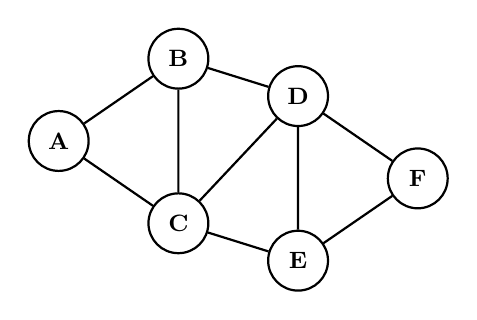
\begin{tikzpicture}[scale=0.95, every node/.style={transform shape}, cv/.style={draw, thick, circle, minimum size=8mm, inner sep=0pt, font=\small\bfseries}]
\node[cv] (A) at (0.00,1.00) {A};
\node[cv] (B) at (1.60,2.10) {B};
\node[cv] (C) at (1.60,-0.10) {C};
\node[cv] (D) at (3.20,1.60) {D};
\node[cv] (E) at (3.20,-0.60) {E};
\node[cv] (F) at (4.80,0.50) {F};
\draw[thick] (A) to[] (B);
\draw[thick] (A) to[] (C);
\draw[thick] (B) to[] (C);
\draw[thick] (B) to[] (D);
\draw[thick] (C) to[] (D);
\draw[thick] (C) to[] (E);
\draw[thick] (D) to[] (E);
\draw[thick] (D) to[] (F);
\draw[thick] (E) to[] (F);
\end{tikzpicture}
\end{adjustbox}
\end{center}
\subq{(a)}\textbf{Cross out} all values that would be eliminated by \emph{forward checking} after variable B has been assigned as shown.\begin{center}\small\begin{tabular}{|l|c|c|c|c|c|c|}\hline Variables & \textbf{A} & \textbf{B} & \textbf{C} & \textbf{D} & \textbf{E} & \textbf{F}\\ \hline Domains & R\ G\ B & \textbf{R} & R\ G\ B & R\ G\ B & R\ G\ B & R\ G\ B\\ \hline\end{tabular}\end{center}

\subq{(b)}A and B have been assigned as shown, but no constraint propagation has been done yet. \textbf{Cross out} all values that would be eliminated by \emph{arc consistency} (AC-3).\begin{center}\small\begin{tabular}{|l|c|c|c|c|c|c|}\hline Variables & \textbf{A} & \textbf{B} & \textbf{C} & \textbf{D} & \textbf{E} & \textbf{F}\\ \hline Domains & \textbf{R} & \textbf{G} & R\ G\ B & R\ G\ B & R\ G\ B & R\ G\ B\\ \hline\end{tabular}\end{center}

\subq{(c)}Variable A is already assigned and constraint propagation has been done. \textbf{Circle} all unassigned variables that might be selected by the \emph{Minimum-Remaining-Values} (MRV) heuristic.\begin{center}\small\begin{tabular}{|l|c|c|c|c|c|c|}\hline Variables & \textbf{A} & \textbf{B} & \textbf{C} & \textbf{D} & \textbf{E} & \textbf{F}\\ \hline Domains & \textbf{R} & G\ B & G\ B & R\ G\ B & R\ G\ B & R\ G\ B\\ \hline\end{tabular}\end{center}

\subq{(d)}Same situation. \textbf{Circle} all unassigned variables that might be selected by the \emph{Degree Heuristic}.\begin{center}\small\begin{tabular}{|l|c|c|c|c|c|c|}\hline Variables & \textbf{A} & \textbf{B} & \textbf{C} & \textbf{D} & \textbf{E} & \textbf{F}\\ \hline Domains & \textbf{R} & G\ B & G\ B & R\ G\ B & R\ G\ B & R\ G\ B\\ \hline\end{tabular}\end{center}

\subq{(e)}Assume no variable has been assigned yet. Solve the CSP using backtracking with \emph{forward checking}, choosing variables with MRV, then the degree heuristic (DH), and finally alphabetical order; try values in the order R, G, B. For every step give the MRV value of every region not yet coloured, and the DH values of the regions tied on the minimum MRV.
\par \underline{Step 1}\par\begin{center}\small \begin{tabular}{|l|c|c|c|c|c|c|}\hline Variables & \textbf{A} & \textbf{B} & \textbf{C} & \textbf{D} & \textbf{E} & \textbf{F}\\ \hline MRV & \phantom{0} & \phantom{0} & \phantom{0} & \phantom{0} & \phantom{0} & \phantom{0}\\[1mm]\hline DH & \phantom{0} & \phantom{0} & \phantom{0} & \phantom{0} & \phantom{0} & \phantom{0}\\[1mm]\hline\end{tabular}\end{center}Assign to the variable \rule{2.5cm}{0.3pt} with the value \rule{2.5cm}{0.3pt}\par
\underline{Step 2}\par\begin{center}\small \begin{tabular}{|l|c|c|c|c|c|c|}\hline Variables & \textbf{A} & \textbf{B} & \textbf{C} & \textbf{D} & \textbf{E} & \textbf{F}\\ \hline MRV & \phantom{0} & \phantom{0} & \phantom{0} & \phantom{0} & \phantom{0} & \phantom{0}\\[1mm]\hline DH & \phantom{0} & \phantom{0} & \phantom{0} & \phantom{0} & \phantom{0} & \phantom{0}\\[1mm]\hline\end{tabular}\end{center}Assign to the variable \rule{2.5cm}{0.3pt} with the value \rule{2.5cm}{0.3pt}\par
\underline{Step 3}\par\begin{center}\small \begin{tabular}{|l|c|c|c|c|c|c|}\hline Variables & \textbf{A} & \textbf{B} & \textbf{C} & \textbf{D} & \textbf{E} & \textbf{F}\\ \hline MRV & \phantom{0} & \phantom{0} & \phantom{0} & \phantom{0} & \phantom{0} & \phantom{0}\\[1mm]\hline DH & \phantom{0} & \phantom{0} & \phantom{0} & \phantom{0} & \phantom{0} & \phantom{0}\\[1mm]\hline\end{tabular}\end{center}Assign to the variable \rule{2.5cm}{0.3pt} with the value \rule{2.5cm}{0.3pt}\par
\underline{Step 4}\par\begin{center}\small \begin{tabular}{|l|c|c|c|c|c|c|}\hline Variables & \textbf{A} & \textbf{B} & \textbf{C} & \textbf{D} & \textbf{E} & \textbf{F}\\ \hline MRV & \phantom{0} & \phantom{0} & \phantom{0} & \phantom{0} & \phantom{0} & \phantom{0}\\[1mm]\hline DH & \phantom{0} & \phantom{0} & \phantom{0} & \phantom{0} & \phantom{0} & \phantom{0}\\[1mm]\hline\end{tabular}\end{center}Assign to the variable \rule{2.5cm}{0.3pt} with the value \rule{2.5cm}{0.3pt}\par
\underline{Step 5}\par\begin{center}\small \begin{tabular}{|l|c|c|c|c|c|c|}\hline Variables & \textbf{A} & \textbf{B} & \textbf{C} & \textbf{D} & \textbf{E} & \textbf{F}\\ \hline MRV & \phantom{0} & \phantom{0} & \phantom{0} & \phantom{0} & \phantom{0} & \phantom{0}\\[1mm]\hline DH & \phantom{0} & \phantom{0} & \phantom{0} & \phantom{0} & \phantom{0} & \phantom{0}\\[1mm]\hline\end{tabular}\end{center}Assign to the variable \rule{2.5cm}{0.3pt} with the value \rule{2.5cm}{0.3pt}\par
\underline{Step 6}\par Assign to the variable \rule{2.5cm}{0.3pt} with the value \rule{2.5cm}{0.3pt}\par
\clearpage
\question{8}\textit{Planning a study session.} You are planning a study session with four decisions: the (S)ubject, the (P)lace, the (T)ime and the (F)ood. The candidates are S $\in\{$\emph{ai, math, phys}$\}$, P $\in\{$\emph{library, cafe, home}$\}$, T $\in\{$\emph{morning, afternoon, evening}$\}$, F $\in\{$\emph{pizza, salad, noodles}$\}$, with the constraints: (1) the library is open only in the morning or afternoon; (2) math must be studied in the morning; (3) pizza is not allowed in the library; (4) AI cannot be studied at the cafe (no sockets).
\subq{(a)}Formulate the problem as a CSP: variables, domains and binary constraints.
\begin{center}\small\begin{tabular}{|l|c|c|c|c|}\hline Variables & \textbf{S} & \textbf{P} & \textbf{T} & \textbf{F}\\ \hline Domains &  &  &  & \\ \hline\end{tabular}\end{center}Binary constraints:\begin{ansbox}[height=1.2cm]\end{ansbox}
\subq{(b)}Draw the constraint graph.
\begin{ansbox}[height=2.6cm]\end{ansbox}
\subq{(c)}You decide to study in the \emph{evening}. Cross out the eliminated values to show the domains after arc consistency has been enforced.
\begin{center}\small\begin{tabular}{|l|c|c|c|c|}\hline Variables & \textbf{S} & \textbf{P} & \textbf{T} & \textbf{F}\\ \hline Domains & ai, math, phys & library, cafe, home & morning, afternoon, evening & pizza, salad, noodles\\ \hline\end{tabular}\end{center}
\subq{(d)}Give one solution, or state that none exists.
\begin{ansbox}[height=0.8cm]\end{ansbox}
\clearpage
\question{9}Answer the following questions briefly.
\subq{(a)}Russell \& Norvig organise definitions of AI into four categories. Name them, state which one this course adopts and give two reasons.
\begin{ansbox}[height=2.6cm]\end{ansbox}
\subq{(b)}Explain the difference between the state space and the search tree, and between tree-search and graph-search algorithms.
\begin{ansbox}[height=2.6cm]\end{ansbox}
\subq{(c)}For a uniform tree with branching factor $b=5$ and the shallowest goal at depth $d=4$, how many nodes does BFS generate in the worst case? Why is memory a bigger problem than time for BFS?
\begin{ansbox}[height=1.8cm]\end{ansbox}
\subq{(d)}Name three landscape features on which hill climbing gets stuck. If one run succeeds with probability $p=0.14$, how many restarts does random-restart hill climbing need on average?
\begin{ansbox}[height=1.5cm]\end{ansbox}
\subq{(e)}Why should variable selection in backtracking be fail-first while value selection is fail-last?
\begin{ansbox}[height=1.8cm]\end{ansbox}
\question{10}True or false?
For each statement, circle \textbf{T} or \textbf{F} and justify your answer in one or two sentences (an answer without a correct justification earns no credit).
\subq{1.}BFS is cost-optimal whenever all action costs are strictly positive. \hfill \textbf{T \quad F}
\begin{ansbox}[height=1.5cm]\end{ansbox}
\subq{2.}Uniform-cost search applies the goal test when a node is generated. \hfill \textbf{T \quad F}
\begin{ansbox}[height=1.5cm]\end{ansbox}
\subq{3.}Every consistent heuristic is admissible. \hfill \textbf{T \quad F}
\begin{ansbox}[height=1.5cm]\end{ansbox}
\subq{4.}If $h_1$ and $h_2$ are admissible, then $\max\{h_1,h_2\}$ is admissible and dominates both. \hfill \textbf{T \quad F}
\begin{ansbox}[height=1.5cm]\end{ansbox}
\subq{5.}Greedy best-first (graph) search is complete in infinite state spaces. \hfill \textbf{T \quad F}
\begin{ansbox}[height=1.5cm]\end{ansbox}
\subq{6.}A poor move ordering may make alpha-beta return a different root value than minimax. \hfill \textbf{T \quad F}
\begin{ansbox}[height=1.5cm]\end{ansbox}
\subq{7.}With perfect move ordering alpha-beta examines $O(b^{m/2})$ nodes. \hfill \textbf{T \quad F}
\begin{ansbox}[height=1.5cm]\end{ansbox}
\subq{8.}In MCTS with UCB1, once a node has children, each of them is selected at least once before any of them is selected a second time. \hfill \textbf{T \quad F}
\begin{ansbox}[height=1.5cm]\end{ansbox}
\subq{9.}Forward checking detects every inconsistency that arc consistency detects. \hfill \textbf{T \quad F}
\begin{ansbox}[height=1.5cm]\end{ansbox}
\subq{10.}In simulated annealing a worse move ($\Delta E<0$) is accepted with probability $e^{\Delta E/T}$, which decreases as $T$ decreases. \hfill \textbf{T \quad F}
\begin{ansbox}[height=1.5cm]\end{ansbox}
\end{document}